\documentclass{article}
\usepackage[utf8]{inputenc}
\usepackage{graphicx}
\usepackage{xfrac}
\usepackage[a4paper, total={6in, 8in}]{geometry}
\usepackage{blindtext}

\graphicspath{/Users/gavinkoma/Desktop/distributed}

\title{Homework 1 \\ Distributed Systems}
\author{Gavin Koma \\ \\ Dr. Jie Wu \\ CIS5644}

\date{February 2nd 2023}

\begin{document}

\maketitle

\newpage
\section{Introduction}
For this assignment, students are required to perform a variety of analyses regarding computing, varying nodes, and logic clocks. These questions are based on the first two lectures of the course and are answered sequentially in order of assignment starting from Exercise 1, Question 2 and progressing with Exercise 2, Question 5. All questions have been retyped to facilitate the grading of this homework. 

\section{Questions}
\textbf{Exercise 1, Question 2: Use your own words to explain the differences between distributed systems, multiprocessors, and network systems.}
\\ \\
1. Distributed systems: \\
A distributed system's main goal is delegate system resources across various hardware. The computer, although built of many connected systems, will generally appear as one computer to the user. 
\\ \\
2. Multiprocessors:\\
A Multiprocessor is a computer system that has two or more central processing units (CPUs). These CPUs will also generally share access to some reservoir of random access memory (RAM). The main objective of these tools is boost the system's speed in regard to executable activities. 
\\ \\
3. Network systems:\\
Network systems is a type of computer operating system that are utilized to support computers. They work to manage the network resources like applications and data and are known to generally ensure security. Some of the most common network systems are Windows Server, Linux, and Max OS X.
\\ \\ \\
\textbf{Exercise 1, Question 3: Calculate (a) node degree, (b) diameter, (c) bisection width, and (d) the number of links for an \textit{n} x \textit{x} 2-d mesh, an n x \textit{n} x \textit{n} 3-d torus, and an \textit{n}-dimensional hypercube.}\\ \\
Let us first perform the calculations for a 2-d mesh. For ease of reading, I have elected to perform all four calculations (a-d) at one time for each individual network viewpoints.\\\\ 
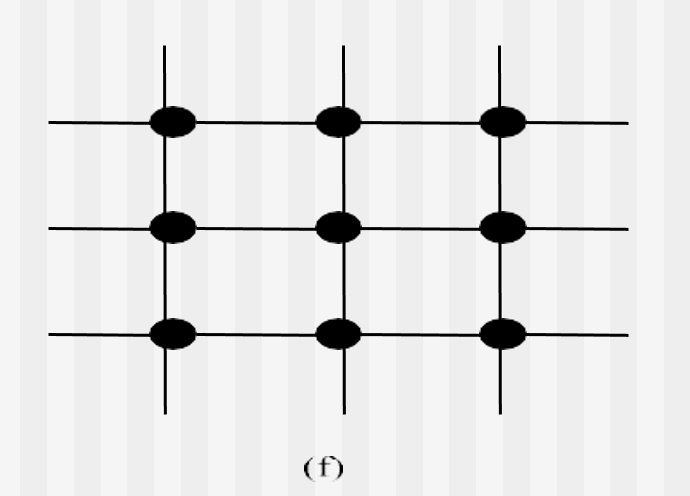
\includegraphics[width=\textwidth,height=\textheight,keepaspectratio]{2dmesh}
\\\\
A node degree is the number of edges incident on a node. An edge is incident on the two nodes upon which it connects. Another important topic to note is that any two nodes connected by one edge or any two edges connected by one node are said to be adjacent. 
\\ \\ 
We can see that each node has a connection above, below, to the left, and to the right. We have not specified the exact dimensions of this mesh other than \textit{n} x \textit{x}. Our book, however, states that a \textit{k}-ary \textit{n}-dimensional mesh will have \textit{N}=\textit{$k^2$}. Thus, a 2-d mesh of \textit{n} x \textit{x} will have
\\ \\
Here we have an \textit{n} x \textit{n} x \textit{n} 3-d torus:\\
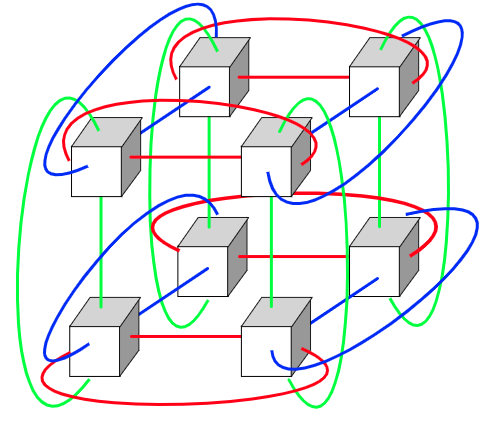
\includegraphics[width=\textwidth,height=\textheight,keepaspectratio]{3dtorus}
\\ \\
A 3-d torus can be referred to as a 3-ary 3-cube network formation. While difficult to imagine, the image depicts a network in which the nodes are placed into a three-dimensional lattice defined in a rectangular prism where each node is connected to its 6 neighbors. Each edge in this formation consists of \textit{n} nodes and communication can take place in all directions of Cartesian coordinate system. The total nodes of a 3-d torus is \textit{$n^3$} while the node degree is 2\textit{n}. The diameter of a 3-d torus can be defined by its dimension \textit{d} and the number of nodes in a given plane \textit{k} by the equation \textit{D}= \textit{d}(\textit{k}-1). Since our torus is 3-dimensional and has four nodes in any given plane, we can confidently say that the diameter is \textit{D}=3(n-1). According to our textbook, a the bisection bandwidth is defined as the bandwidth available between two equally partitioned sections. A 3-d torus of n nodes would have $\sfrac{n^2}{2}$. Finally, we calculate the number of links. For a 3-d torus, this is performed by calculated \textit{$n^3$}.
\\ \\
Finally, we have an \textit{n}-dimensional hypercube. Attached below is a graphic for reference:
\\ 
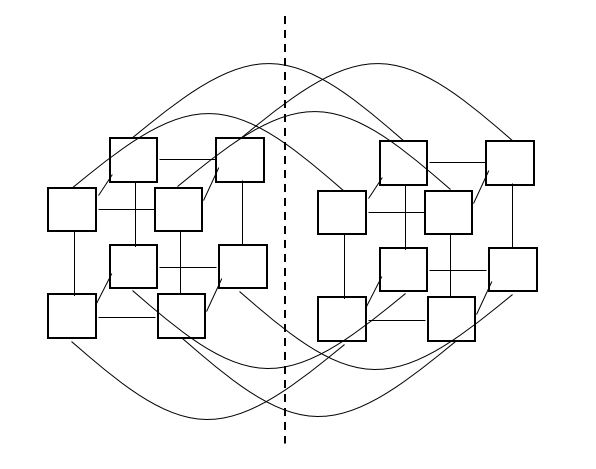
\includegraphics[width=\textwidth,height=\textheight,keepaspectratio]{hypercube.jpeg}
\\ \\
Again, we must calculate the node degree, diameter, bisection width, and the total number of links. A hypercube is generally considered a method to connect multiple processors with multiple memory modules and have the ability to efficiently stream data. \\ \\ 
A hypercube consists of \textit{N} = \textit{$2^m$} nodes which are actually formed by the vertices of the 8 three-dimensional cubes that comprise its facets. It is important to note that while the nodes of a hypercube are \textit{N} = \textit{$2^m$}, m is the number of bits that are \textit{required} to label the nodes in the network. One way to think this through is to consider a situation in which \textit{N} = 4. In this case, 2 bits are required to represent every node in then network; Thus, 4 = $2^2$. \\ \\ 
Next, we must consider the diameter of an \textit{n}-dimensional hypercube. The diameter can be defined as the maximum number of nodes that a message \textit{must} pass through to get to its destination. The general diameter for an \textit{n}-dimensional hypercube is defined by m (the number of bits). \\ \\
The bisection width of a hypercube in terms of internetwork topology is the lowest number of wires that one would have to cut in order to divide our network into two equal halves. This is the same as it has been for all previous definitions of diameter for this assignment. For a hypercube, this is defined by $2^{(m-1)}$.\\ \\
Finally, we calculate the total number of links. This could appear as trickey for something so dimensionally-confusing \textit{n}-dimensional however, multiple recent papers say that the total number of links in an \textit{n}-dimensional hypercube is 0.5*($2^n$)(n). 
\\ \\ \\
\textbf{Exercise 2, Question 2: For the distributed system shown in the figure below.}
\\ \\
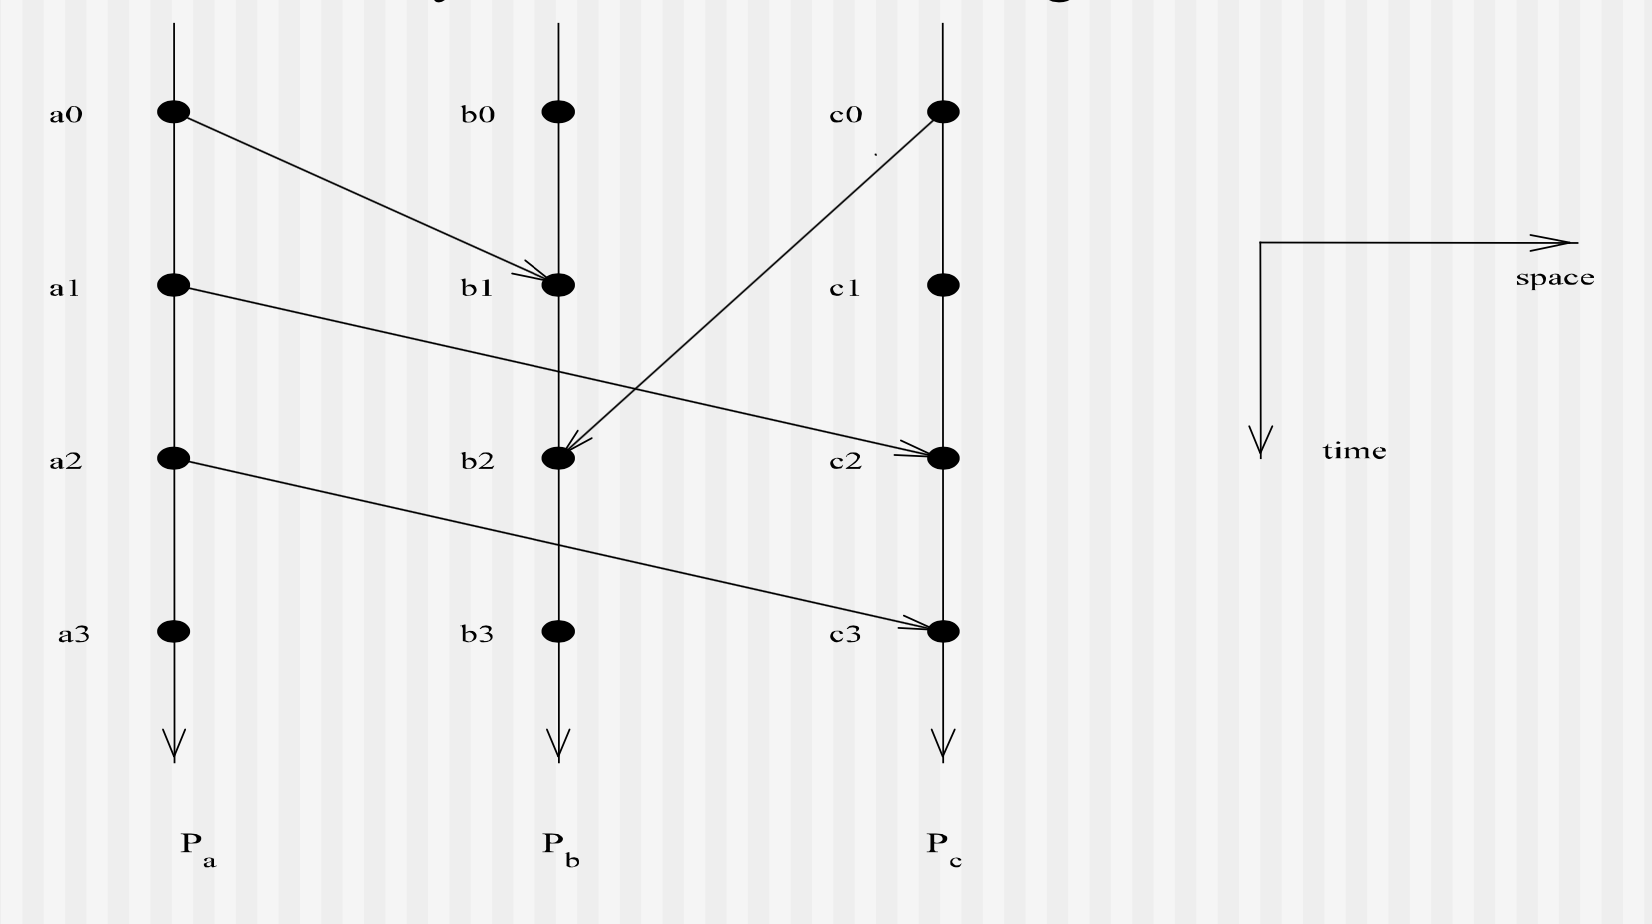
\includegraphics[width=\textwidth,height=\textheight,keepaspectratio]{q2}
\\ \\
\textbf{Provide all the pairs of events that are related.}
\textbf{Provide the logical time for all events using: (a) linear time and (b) vector time; assume that each \textit{$LC_i$} is initialized to zero and the \textit{d}=1.}\\ \\
Instead of typing these values myself, for ease of reading and sake of brevity, I have edited the diagram to have the values for linear time and vector time onto the diagram. I have included two separate images: Image A for linear time and Image B for vector time. \\ \\ \\ \\ \\ \\ \\ \\ \\ \\ \\ \\ \\ \\ \\
Image A: \\ \\ 
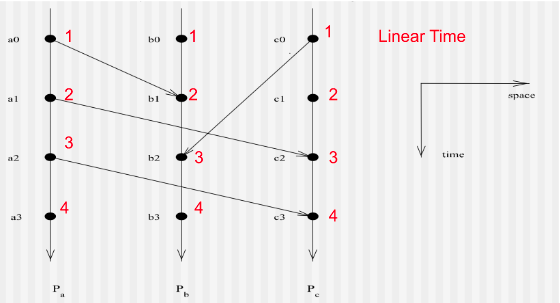
\includegraphics[width=\textwidth,height=\textheight,keepaspectratio]{linear.png} \\ \\
Image B: \\ \\
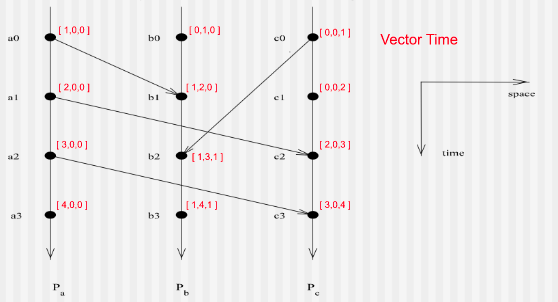
\includegraphics[width=\textwidth,height=\textheight,keepaspectratio]{vector.png}
\\ \\ \\
\textbf{Exercise 2, Question 3: Provide linear logical clocks for all the events in the system given in Problem 2. Assume that all \textit{LC}'s are initialized to zero and the \textit{d}'s for \textit{$P_a$}, \textit{$P_b$}, and \textit{$P_c$} are 1, 2, and 3, respectively. Does condition \textit{a}$\,\to\,$\textit{b} $=>$ \textit{LC(a)} $<$ \textit{LC(b)} still hold? For any other set of \textit{d}'s? and why?} \\ \\ 
To begin this problem, we will view the same same graph but consider varying values of $d$. The linear clock values are as follows: \\ \\
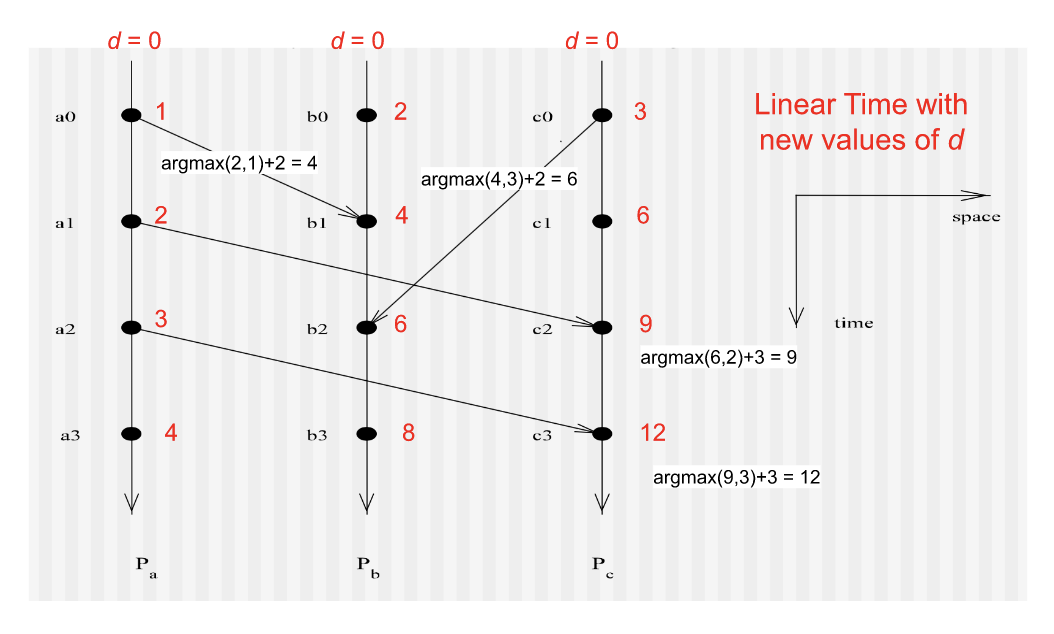
\includegraphics[width=\textwidth,height=\textheight,keepaspectratio]{new_d.png}\\ \\
As with any logical clock, the condition that \textit{a}$\,\to\,$\textit{b} $=>$ \textit{LC(a)} $<$ \textit{LC(b)} will hold true if the event $a$ that occurs before event $b$ has a logical clock value in which the value of event $a$ is less than the value of event $b$. This is the requirement of this condition as it \textit{must} reflect the correct order of events within the computer system.\\ \\
This example specifies varying values of distance ($d$) such that \textit{$P_a$}, \textit{$P_b$}, and \textit{$P_c$} are 1, 2, and 3, respectively. Here, \textit{$P_a$} is incremented by a distance value of 1 and \textit{$P_b$} is incremented by a distance value of 2. In this case, we can be assured that \textit{LC(a)} $<$ \textit{LC(b)} as shown. These conditions would continue to hold for any value of $d$ if $d$ is a positive value. However, if any of these $d$'s were to be a negative integer, it is likely that our logical clock values would falter and the conditions would not be upheld. 
\\ \\ \\
\textbf{Exercise 2, Question 4: Traversal on graph \{(a,b), (b,c), (b,d), (c,e), (d,e), (e,f)\} using Terry's solution and Awerbuch's extension.}
\\ \\ \\
To begin this problem, I created a graph that shows the traversals described in the previously described matrix: \\\\
\centerline{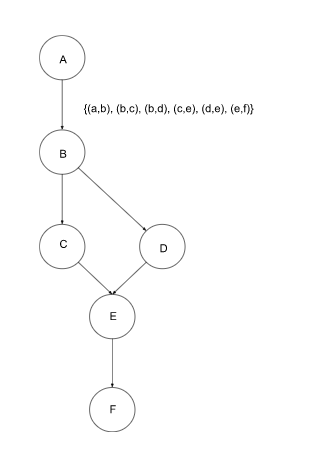
\includegraphics[width=70mm,scale=0.7]{graph.png}} \\ \\
$Terry's$ $Solution$ is a depth-first search (DFS) algorithm that implements a label in order to keep track of each node and its corresponding parent. The algorithm works by beginning at the root node and keeps a record of all nodes as it progresses through its traversal. The algorithm visits each child node in a depth-first manner and will only backtrack if the final node has no children. If so, the algorithm will backtrack to its parent. For this graph, the traversal using $Terry's$ $Solution$ would result in \textit{A}$\,\to\,$\textit{B}$\,\to\,$\textit{C}$\,\to\,$\textit{E}$\,\to\,$\textit{F}. At node $F$, the algorithm would backtrack to node \textit{B} and progress to node \textit{D} (instead of C) and then backtrack to the root node (node \text{A}).\\ \\
$Awerbuch's$ $Extension$ is another depth-first search algorithm that builds on $Terry's$ $Solution$ but it will act to store state conditions of the algorithm as it progresses through each node. If a node at some point were temporarily unavailable, the algorithm would resume the traversal again from that unavailable node. Essentially, if for some reason, node $B$ became temporarily unavailable, the algorithm would store the state condition of that ndoe and continue the traversal again from that node when it becomes available. 
\end{document}